\section{Experiment}
\label{sec:exp}

The micromegas and scintillator detectors of the Harvard cosmic ray test stand are described in detail in previous notes presenting the performance of the full MMFE8 readout~\cite{noisy,noiseless}. Eight layers of micromegas detectors are stacked vertically for the purpose of providing eight measurements of the position of a cosmic muon as it travels through the experiment. The readout strips of each layer have a pitch of 0.4 mm, and they are arranged as designed for the NSW: $XXUVUVXX$, where strips in the $X$ planes run perpendicular to the readout edge of the chamber, and strips in the $U$ ($V$) planes are tilted at an angle of $1.5^\circ$ ($-1.5^\circ$) to provide a measurement of the non-precision coordinate. Each layer of micromegas is 20 cm by 20 cm.

Three layers of scintillators with PMTs for light detection are placed above, on top of, and below the micromegas to provide a trigger for the full MMFE8 readout. A scintillator trigger is formed when all three layers of scintillator detect a coincidence. There is $\sim\!2\!-\!3$ meters of concrete between the micromegas and the bottom scintillator to filter low-energy particles.

\subsection{Electronics}
\label{sec:exp-elx}

The micromegas readout paths includes three separate cards. The MMFE8 is the front-end readout card, and it houses 8 VMM2 ASICs per card. These readout chips receive signals from the detector and digitize them, and they are discussed in great detail elsewhere~\cite{nswtdr,noisy,noiseless}. The MMFE8 also houses an FPGA for configuring and reading out the VMMs over ethernet. The experiment in this note has 8 layers of micromegas detectors and therefore 8 MMFE8s.

The ART Data Driver Card (ADDC) is a driver card for the micromegas trigger data path. It receives data from 4 MMFE8s over mini-SAS connections and packages this data into a single output for downstream clients. The card houses an FPGA for this purpose. There are 2 ADDCs in this experiment to receive data from the 8 MMFE8s.

The Micromegas Trigger Process (MMTP) is the last card of the micromegas trigger path. It receives data from ADDCs over fiber optical connections and interrogates the data for the presence of triggers. The card houses an FPGA for this purpose. There is 1 MMTP in this experiment to receive data from the 2 ADDCs.

Additionally, a board was built at Harvard for the purpose of operating the MMFE8s synchronously, referred to as the clock/trigger board. This board sends a 40 MHz clock to all 8 boards, which are used by each board as a mother clock, thereby synchronizing them. The board also receives trigger signals from the scintillator and distributes them to the MMFE8s, as discussed in Section~\ref{sec:exp-mmfe}. A cartoon schematic of the electronics is shown in Figure~\ref{fig:cartoon_elx}.

\begin{figure}[!htpb]
  \begin{center}
    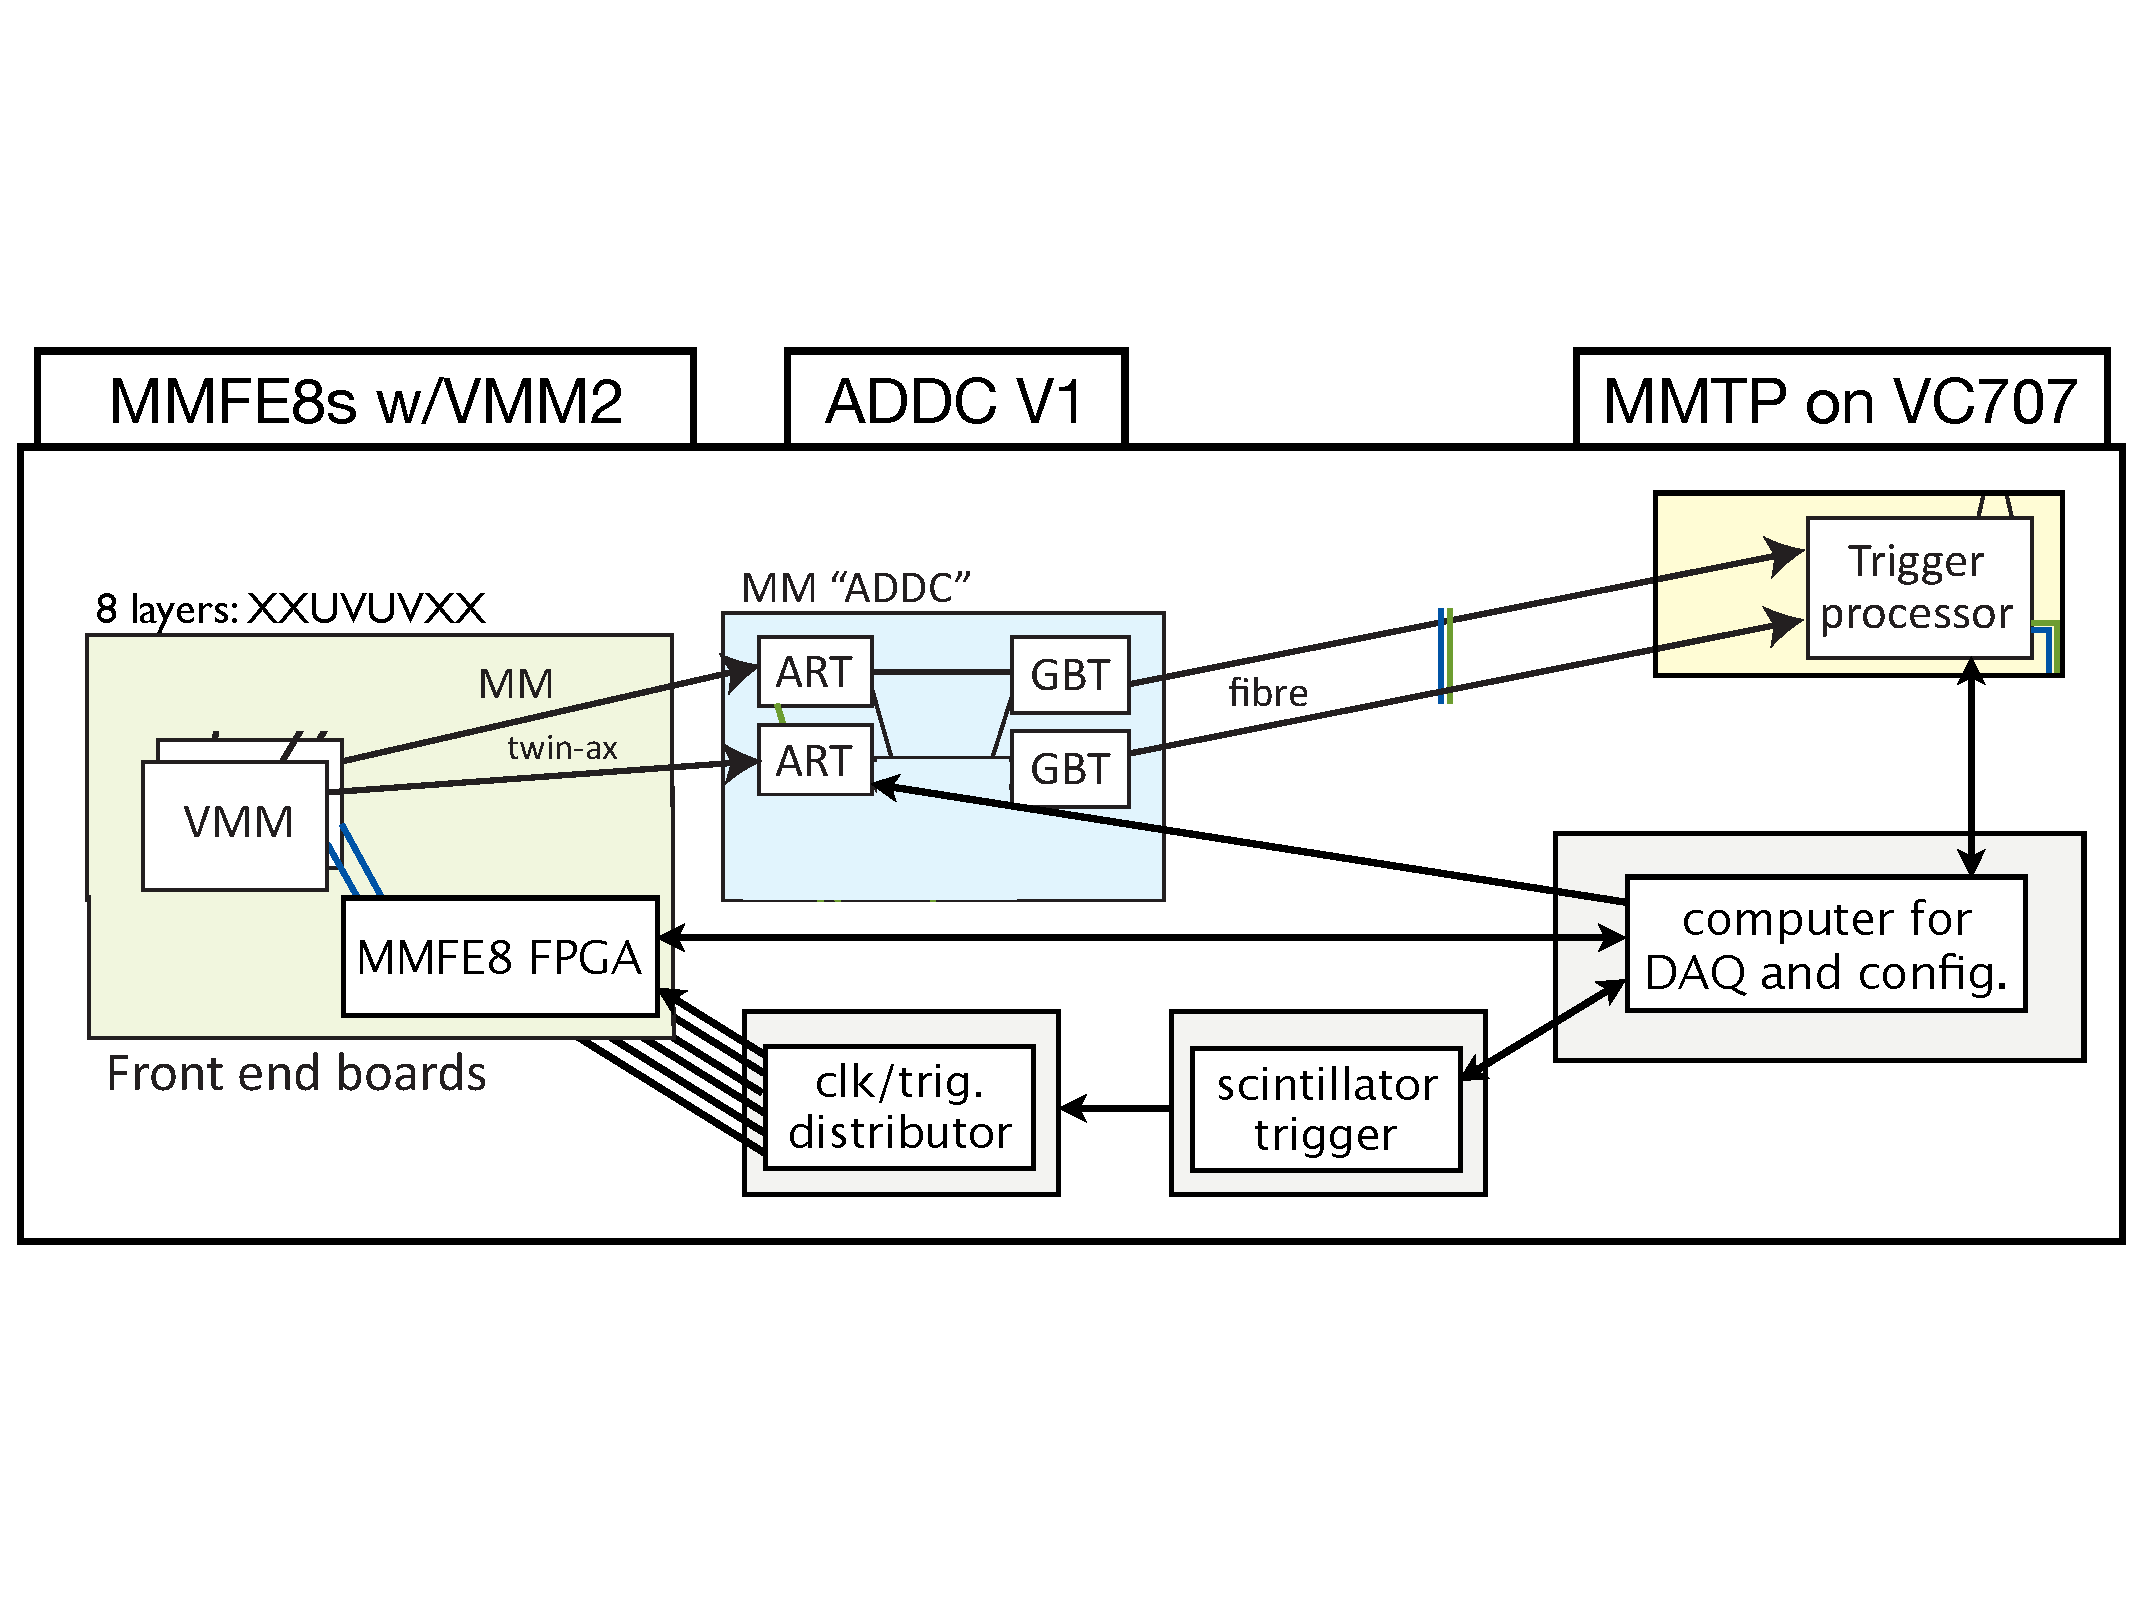
\includegraphics[width=1.0\textwidth]{figures/cartoons/electronics_path.pdf}
  \end{center}
  \vspace{-20pt}
  \caption{Cartoon schematic of the data flow in the electronics used at the Harvard cosmic ray test stand. Inspiration for the cartoon is provided by L. Levinson.}
  \label{fig:cartoon_elx}
\end{figure}

\subsection{Trigger data path}
\label{sec:exp-art}

The micromegas trigger data path begins at the VMM. The data path is referred to as the Address in Real Time (ART) data path, which refers to the output of the VMM. The full readout can include many strips per BC, and each strip read out includes lots of information about the strip, including charge (PDO) and time (BCID, TDO). Alternatively, the trigger readout sends the data from at most one strip per BC, and it only includes the address of the strip. This is the crux of the trigger data path; the bandwidth of the trigger data path is greatly reduced relative to the full readout. One bit is used to announce a hit is recorded, and six bits are used for the address.

The VMM has two operating modes for the ART: at-threshold and at-peak. These modes describe the time at which an ART signal is sent by the VMM. Threshold mode is faster than peak mode because the VMM sends the signal as soon as a threshold is crossed, instead of waiting until a peak is found. The data in this note are taken with the ART operating at threshold.

The VMM sends ART data over mini-SAS cables to the ART Data-Driver Card (ADDC), which collects ART signals from 4 MMFE8 and packages them into a single output. The ART data bypasses the MMFE8 readout chip entirely. The data in this note are taken with ADDC V1, in which the ADDC has an on-board FPGA for collecting and packaging the incoming signals. The final version of the ADDC will have an on-board ASIC for this purpose, since it will be mounted in the ATLAS cavern and must be radiation tolerant. However, the functionality of the FGPA-based and ASIC-based ADDC are expected to be identical.

The ADDC then sends the packaged ART data to the micromegas trigger processor (MMTP). The communication protocol is ``GBT'', which is developed at CERN and used by many experiments, and sent over fiber optic cables. The MMTP collects ART signals, analyzes them for patterns resembling a trigger, and sends trigger information to downstream clients. These steps are performed by an FPGA. The data in this note are taken with an implementation of the MMTP on a Xilinx VC707 development board with a Virtex-7 FPGA.

In this setup, 2 ADDCs are placed near the detector and accept ART signals from the 8 MMFE8s. The VC707 is placed further from the detector in a counting room, along with the DAQ computer and scintillator readout electronics. It accepts signals from both ADDCs.

\subsection{MMFE8 and scintillator data path}
\label{sec:exp-mmfe}

The MMFE8 and scintillator data paths are described in detail elsewhere~\cite{noisy,noiseless}. In brief, the DAQ computer communicates directly with the MMFE8s over ethernet connection. The full MMFE8 readout includes charge and time information for each strip above threshold in the form of PDO, TDO, and BCID. The MMFE8 only sends data over ethernet after it has received a trigger signal from the scintillator. The signal is sent from the scintillator to the clock/trigger board over coaxial cable with BNC connections, and the clock/trigger board sends this signal to the 8 MMFE8s over microHDMI.

The scintillator trigger is formed with a coincidence of six signals corresponding to the top, middle, and bottom scintillator counters. The signals are acquired by Lecroy TDC and sent to a CAMAC crate controller, which then sends its data over ethernet to the DAQ computer.

\subsection{Scintillator timestamp}
\label{sec:exp-scitime}

Additionally, there is a connection between the scintillator electronics and the MMTP, to utilize the fast internal clocks of the MMTP FPGA. The scintillator trigger signal is sent directly to the MMTP, which captures the signal using a 640 MHz clock and forwards this timestamp to the DAQ computer over ethernet. This is referred to as the \textit{scintillator timestamp}. It provides a more accurate reference time than the scintillator BCID captured by the MMFE8s, since the 640 MHz clock of the MMTP allows for $\sim\!1.56$ ns resolution, versus the $\sim\!25$ ns resolution of the 40 MHz clock.

